Evolutionary psychologists are interested in personality because there are clues that suggest it might play an important role in natural selection. The first such clue is that much research shows personality to exhibit stability over time and contexts\mcite{cooper2015individual, larsen2008personality, buss2009can}. The second is that studies have shown individual personality traits to be $30-50\%$ inherited\mcite{newman1998individual, THG:8492454}. This strongly suggests that there are fitness benefits to different genetically inheritable aspects of personality.
EP suggests that due the heredity of personality it may be seen, from an evolutionary point of view, as \textbf{a type of behavioral strategy}, i.e. a motivational system which predisposes people to seek out particular situations and respond in particular ways\mcite{workman2014evolutionary}.
This argumentation, however, gives rises to a paradox: in trying to explain the heredity of personality traits by assuming that the traits increase fitness, the question of why personality is \textit{only} $30-50\%$ genetic must be addressed.
EP has several theories to explain this, of which the two central ones are: (1) the brain develops as it does due to \textit{chance} because the genome only contains \textasciitilde20,300 genes of information which cannot possibly code exactly for a brain that has \textasciitilde100 billion complexly interacting neurons and (2) the individual is born with an adapted capacity for environmental calibration because inherent uncertainty of the world renders a fixed strategy on birth suboptimal\mcite{workman2014evolutionary}.

% Personality is treated as a strategy in large part because it conveniently explains empirical observations, but there are no and as such it should be considered a \textit{hypothesis}, which is a notion that should be respected when using this view as a basic assumption for further research. In fact, key founders of EP, Leda Cosmides and John Tooby, argued in an early paper (1990) that heritable individual differences are simply noise irrelevant to the basic functioning of the psychological machinery, similar to how the color of wires in a car engine have no effect on the actual functioning of the car\mcite{tooby1990universality}. This view has changed today. High-profile evolutionary psychologist and linguist Stephen Pinker openly talks about personality as strategy in his acclaimed book \textit{How The Mind Works} (1999}\mcite{pinker1999mind}, and the most cited personality researchers in EP David Buss and Daniel Nettle are firmly dedicated to this view\mcite{buss2009can, nettle2006evolution}.

EP's primary instrument for measuring personality is the BFM because, as argued by Buss, it represents the most evolutionarily plausible way of carving up human personality\mcite{buss1991evolutionary, larsen2008personality}. The main reason for this is because the traits are orthogonal and they capture a wide array of individual differences. To compare, in one end of the scale Cattell's 16PF model elaborately cover many aspects of personality at the cost of using a very non-orthogonal system of traits, whereas in reverse the Eysenck model is too narrow and disregards evolutionarily important traits like \textit{agreeableness}, \textit{conscientiousness} and \textit{openness to experience}.

% Trade-offs
\subparagraph*{Trade-offs cause trait variations}
Trade-offs between physical and psychological traits are inherent to almost all biological systems. It can be understood intuitively as the problem of having to choose between things that are good for something but can't be had simultaneously. Like being big or small: each has advantages, but obviously an organism must somehow choose to be either like one or a \textit{trade-off}. An investigated example from Darwinian evolutionary theory explains the practical value of this problem. 
Ground finches on the Galapagos are typically sectioned into three types: (1) long beak/medium body, (2) large thick beak/large body and (3) small thick beak/small body. Shoval et. al. shows that each of these trait configurations are in fact archetypes of traits exhibited by all ground finches, and that each archetype is optimized to perform a specific task (see Figure \ref{fig:trade_offs_finch_paretoOptimality}.b)\mcite{shoval2012evolutionary}. Archetype-(1) is optimized for picking insects and extracting nectar, archetype-(2) is optimized for cracking large hard seeds and archetype-(3) is optimized for crushing small soft seeds. Shoval et. al. observes that most ground finches are, however, not exactly like any archetype, rather each seems to \textit{trade off} archetypal traits such as to be able to perform all tasks to some ability. This is thought to be a strategy for coping with changing ecological pressures, such that when a niche becomes unavailable (e.g. small soft seeds disappear) the organism has other ways of leveraging its fitness.

\begin{figure}[ht]
	\centering
	\textbf{a)}
	\hspace{0.2cm}
	\begin{minipage}[r]{0.4\textwidth}
		\centering
		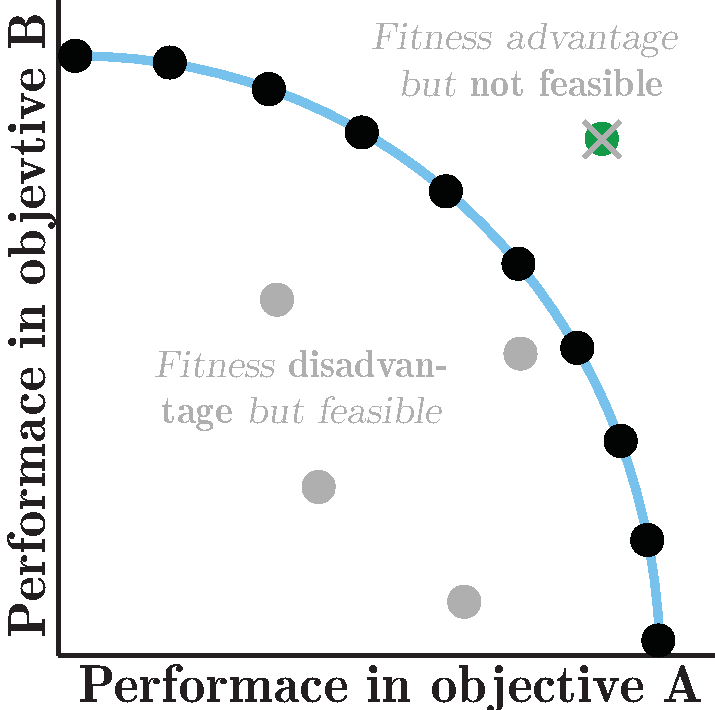
\includegraphics[width=1\textwidth]{figures/paretoOptimality}
	\end{minipage}
	\hspace{0.7cm}
	\textbf{b)}
	\hspace{0.2cm}
	\begin{minipage}[l]{0.4\textwidth}
		\centering
		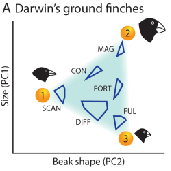
\includegraphics[width=1\textwidth]{figures/trade_offs_finch}
	\end{minipage}
	\caption{\label{fig:trade_offs_finch_paretoOptimality} \textbf{a)} Illustration of distribution of points in a two-objective performance space where the black points are Pareto optimal and the blue curve signify the Pareto front where no objective can be optimized further without decreasing performance in the other. \textbf{b)} Illustration of how members of a species is distributed in trait-space to respect trade-offs between archetypal traits (source: Shoval et. al.\cite{shoval2012evolutionary}).}
\end{figure}

It is reasonable to ask what the best trade-off configuration of traits is, but the immediate answer is that there are infinite. To explain what this means, the concept of \textit{Pareto optimality} must be introduced. Pareto optimality is a concept that stems from Economics and characterizes the set of solutions to a multi-objective optimization problem where no objective can be further optimized without having to compromise performance of another. For two objectives this means that solutions that are Pareto optimal are distributed along a curve in performance space, as illustrated in Figure \ref{fig:trade_offs_finch_paretoOptimality}.a. For an individual organism, traits will be adopted in such a way the the organism remain Pareto optimal, i.e. good enough at all evolutionarily important tasks to remain fit. Those that are not on the Pareto front will have a fitness disadvantage and be selected against in the long run, thus not passing on the genes that caused the disadvantage. The propensity to seek niches of least competition, i.e. \textit{Niche filling}, drives populations to distribute traits somewhat evenly across the Pareto front.

The configuration of traits that a ground finch inherits from its parents can, in an evolutionary view, be considered a \textit{strategy} for coping with the environment. This view is conceptually similar to the way evolutionary psychologists treat personality. For this reason, an individuals configuration of personality traits is also considered to be under influence of trade-offs. For example a person cannot (disregarding personality disorders) be both extroverted and introverted at the same time, and if life in general can be viewed as a complex collection of tasks then a persons level of intro-/extraversion poses an evolutionary trade-off problem just as much as beak shape does to seed-cracking.

\subparagraph*{Frequency dependence drives emergence of multiple strategies}
EP treats the predominance of different personalities/behavioral strategies using the concept of \textit{frequency dependence} from evolutionary theory. It argues that the reason why all humans have not simply adapted the \textit{single best strategy} is that, while at times there may be one strategy which is the best, this quickly changes when too many individuals adopt it. This can be compared to how driving to work early is a good strategy for avoiding traffic as long as not too many people do it. Another example is that of \textit{psychopathy}. Workman et. al. argues that psychopathy is in fact (purely evolutionarily speaking) a very effective behavioral strategy to maximize personal fitness \footnote{Also: \textit{exclusive fitness} - only increasing fitness of self as opposed to \textit{inclusive} fitness which measures fitness of all kin.}, provided there are not too many psychopaths around\mcite{workman2014evolutionary}. In most populations only 1-3\% of individuals will adopt this strategy to a sub-clinical level whereas clinical psychopathy is as low as 0.2\%\mcite{kring2005abnormal}. The psychopath strategy revolves around gaining peoples trust and then using them for own goals, and imaginably this strategy wouldn't work well if there were so many psychopaths that otherwise trusting people were used to getting cheated by psychopaths and therefore in general learned only to trust kin or long-term friends.

\newcommand*\rot{\rotatebox{90}}
\newcommand*\OK{\ding{51}}
\newcommand{\lbo}[1]{\multicolumn{1}{|c|}{#1}}
\newcommand{\rbo}[1]{\multicolumn{1}{c|}{#1}}
\newcommand\Tstrut{\rule{0pt}{4ex}}
\newcommand\Bstrut{\rule[-1.9ex]{0pt}{0pt}}
\newcommand{\playerA}{\multirow{2}{*}{\rotatebox{90}{\textbf{You}}}}
\begin{table}
	\vspace{-0.75cm}
	\centering
	\begin{minipage}[l]{0.49\textwidth}
		\hspace{-0.5cm}
		\begin{tabular}{R{0.1cm}C{0.9cm}C{1.5cm}C{1.5cm}}
			{} 		& {}	& \multicolumn{2}{c}{\textbf{Opponent}} \vspace{0.15cm}\\
			{} 		& {}	& \multicolumn{1}{C{1.5cm}}{Hawk}& 	\multicolumn{1}{C{1.5cm}}{Dove}	\\ \cline{3-4}
			\playerA& Hawk	& \lbo{$(V-C)/2$} 	& \rbo{$V$} 	\Tstrut\Bstrut					\\ \cline{3-4}
			{} 		& Dove	& \lbo{0} 			& \rbo{$V/2$} 	\Tstrut\Bstrut\Bstrut			\\
			\cline{3-4}
		\end{tabular}
	\end{minipage}
	\hspace{0.1cm}
	\begin{minipage}[r]{0.45\textwidth}
		\vspace{1.4cm}
		\caption{\label{tab:prisoners_dilemma} Reward table for the hawk-dove game. It models an exchange between 'you' and an opponent where each chooses e.g. to be like a dove (cooperate) or hawk (cheat). Each combination of moves has a different reward for each player.}
	\end{minipage}
	\vspace{-0.25cm}
\end{table}

\subparagraph*{Game theory can explain some behavioral strategies}
The suggestion that personality is a behavioral strategy must be understood in terms of what evolutionary psychologists already identify with the term 'strategy'. It has its roots in the field of game theory, which examines how people behave depending on the strategies of others. Here the term is simply synonymous with \textit{algorithm}. A central goal of applying game theory is to find a strategy for an individual which, given what everybody else is doing, cannot make the individual better off. Such as strategy is said to represent a state of \textit{Nash Equilibrium}. A commonly treated paradigm is the so-called \textit{hawk-dove game} which is illustrated in Table \ref{tab:prisoners_dilemma}.
It models an interaction between two players, \textit{you} and an \textit{opponent}, who have to share a resource $V$. Each player can choose to cooperate or defect, i.e. act as a \textit{dove} or as a \textit{hawk}. If both cooperates $V$ is shared equally, but if one chooses to cooperate while the other doesn't the gullible player gets nothing while the defector gets all. In case both players choose the hawk-strategy the resources are shared equally but at the cost of battle, $C$. This game has been studied extensively, and for repeated games - between rational players - the winning strategy is a so-called \textit{tit-for-tat} strategy\mcite{workman2014evolutionary}, where one simply copies the opponents' last move. This strategy constitutes a Nash equilibrium because, provided the opponent doesn't change strategy, there is nothing to gain from changing strategy\mcite{nash1950equilibrium}. Other strategies such as a \textit{generous-tit-for-tat} which chooses cooperation with some probability even if the opponent has defected, or \textit{win-stay lose-shift} which (even simpler) just repeats past moves if they were successful and tries something new if not, have been shown to work slightly better when the opponent acts irrationally\mcite{nowak2006five}. Other less sophisticated strategies which are not in equilibrium are \textit{uncompromising cooperation} as well as \textit{constant defecting}.

A generalization of the Nash equilibrium to describe evolutionary stability which is used in biology, behavioral ecology and EP is the concept of the evolutionarily stable strategy (ESS). An ESS is a behavioral strategy that, if it exists abundantly enough in a population, it cannot be replaced by an invading strategy\mcite{smith1974theory}. It links to the concept of frequency dependence examined above, when multiple ESSs exist alongside, because they depend on each other in complex ways (recall the example with psychopathy), and can therefore be said to be \textit{inter}-frequency dependent (this terminology is not used in literature but resonates with notions raised by Workman et. al.\mcite{workman2014evolutionary} and Buss \mcite{buss2009can}).

EP considers a number of behavioral strategies to be ESS. Firstly the psychopathy strategy is thought to be ESS. Another is \textit{reciprocal altruism} which has been extensively studies in tribe cultures\mcite{workman2014evolutionary}, where individuals tend to give presents to non-kin with the expectation that presents will be returned to them at another time of greater need. Reciprocal altruism is formally treated as either: (1) \textit{direct} where reciprocity is expected from the same person/group and of equal value as was donated (compared to the tit-for-tat strategy) or (2) \textit{indirect} which relies on good reputation, established through gossip of altruistic acts, to eventually provide the giver with resources from like-minded (cooperation strategy)\mcite{nowak2006five}.
Another important strategy which is thought to be ESS is the \textit{freeloader}, which utilizes the cooperators trusting nature to cheat as frequently as possible within the limit of remaining an ESS. Evolutionary psychologists speculate the \textit{freeloader} to have significant importance to community formation through exemplifying morally wrong behavior\mcite{workman2014evolutionary}.

% \textbf{Individual personality is a trade-off between fundamental strategies}.
% To fully adapt one fundamental strategy is rarely a robust solution due to the fitness fluctuations that result from frequency dependence.
% An individual will therefore tend to adopt a strategy that is a mix of many fundamental strategies.
% This can be thought of as a multi-objective optimization problem: individuals must ensure maximal fitness but adopted strategies must obey inherent trade-offs between performance of fundamental strategies.
% It confines solutions to a surface in performance space called the \textit{Pareto front}.
% The Pareto front defines the boundary where increasing performance in one strategy comes at the expense of performance in others.
% Evolution tends to not allow individuals to stay off the Pareto front because their fitness advantage would be inferior to those on it, and as such personalities of people should be confined to the Pareto front where they remain \textit{Pareto optimal} trade-offs between fundamental strategies.